
%%%%%%%%%%%%%%%%%%%%%%% file typeinst.tex %%%%%%%%%%%%%%%%%%%%%%%%%
%
% This is the LaTeX source for the instructions to authors using
% the LaTeX document class 'llncs.cls' for contributions to
% the Lecture Notes in Computer Sciences series.
% http://www.springer.com/lncs       Springer Heidelberg 2006/05/04
%
% It may be used as a template for your own input - copy it
% to a new file with a new name and use it as the basis
% for your article.
%
% NB: the document class 'llncs' has its own and detailed documentation, see
% ftp://ftp.springer.de/data/pubftp/pub/tex/latex/llncs/latex2e/llncsdoc.pdf
%
%%%%%%%%%%%%%%%%%%%%%%%%%%%%%%%%%%%%%%%%%%%%%%%%%%%%%%%%%%%%%%%%%%%


%\documentclass[runningheads,a4paper]{llncs}
\documentclass[a4paper]{./plantillas/llncs}

\usepackage{amssymb}
\setcounter{tocdepth}{3}
\usepackage{graphicx}

\usepackage{url}
\urldef{\mailsa}\path|{jmanuel, gonzalo}@bacchuss.biz|    
\newcommand{\keywords}[1]{\par\addvspace\baselineskip
\noindent\keywordname\enspace\ignorespaces#1}

%JMANUEL
\usepackage[utf8]{inputenc}  %con el formato de applemac no andan los acentos directos.
\usepackage[spanish]{babel}

%JMANUEL NOTAS:
% Para poner txt en itálicas: \emph{palabra}



\begin{document}

\mainmatter  % start of an individual contribution

% first the title is needed
\title{VIDIX - Detección Visual de Intrusos en Redes de Datos}

% a short form should be given in case it is too long for the running head
%\titlerunning{Lecture Notes in Computer Science: Authors' Instructions}

% the name(s) of the author(s) follow(s) next
%
% NB: Chinese authors should write their first names(s) in front of
% their surnames. This ensures that the names appear correctly in
% the running heads and the author index.
%
\author{Juan Manuel Ramon Mosso, Gonzalo Buszmicz}
%
\authorrunning{Lecture Notes in Computer Science: Authors' Instructions}
% (feature abused for this document to repeat the title also on left hand pages)

% the affiliations are given next; don't give your e-mail address
% unless you accept that it will be published
\institute{Bacchuss, Investifación y Desarrollo,\\
Sarmiento 537 PB B., 2000 Rosario, Santa Fe, Argentina\\
\mailsa\\
\url{http://www.bacchuss.biz}}

%
% NB: a more complex sample for affiliations and the mapping to the
% corresponding authors can be found in the file "llncs.dem"
% (search for the string "\mainmatter" where a contribution starts).
% "llncs.dem" accompanies the document class "llncs.cls".
%

\toctitle{Lecture Notes in Computer Science}
\tocauthor{Authors' Instructions}
\maketitle


\begin{abstract}
La dependencia en las TIC como uno de los pilares fundamentales para el desarrollo social, económico y militar, junto a la tendencia acentuada en el número de redes y servicios conectados a Internet, generan un incremento considerable en los niveles de riesgo de seguridad asociados a los datos y servicios de TI. Los atacantes encuentran en este tipo de escenario un gran abanico de oportunidades para alcanzar sus objetivos debido a la gran diversidad y complejidad de los sistemas intervinientes los cuales son inexorablemente sujeto de vulnerabilidades. Las consecuencias de un ataque exitoso incluyen entre otros, interrupción de servicios, robo o alteración de información, etc., lo que en algunos casos puede derivar en verdaderas situaciones de crisis con gran impacto. El escenario descripto presenta un contexto altamente desafiante para los analistas de seguridad involucrados en los diferentes procesos involucrados en la gestión de incidentes de seguridad debido a la gran cantidad y diversidad de datos a procesar, y de herramientas, procesos y conocimiento necesarios para resolver la problemática de manera eficaz y eficiente.

Para avanzar en una solución al problema se plantea el desarrollo de un sistema de representación gráfica basado en técnicas de análisis visual y fusión de datos que permita alcanzar un estado de comprensión de que es lo que esta sucediendo a nivel de seguridad. A este estado de comprensión de todos los componentes y variables intervinientes se lo conoce como Conocimiento de la Situación (CS). El proceso de CS resulta fundamental como soporte de toma de decisiones para diferentes áreas de aplicación como por ejemplo para el control aéreo, el manejo de crisis, etc. En este caso se utilizará el CS con el objetivo de optimizar el proceso de comando y control en el contexto de seguridad de la información. \newline 

{\bfseries Palabras clave:} análisis visual, fusión de datos, seguridad, redes de datos 

\end{abstract}



\section{Introducción}

La dependencia en tecnologías de información y comunicaciones como uno de los pilares fundamentales para el desarrollo social, económico y militar de las naciones y corporaciones,  junto a la tendencia acentuada en el número de redes y servicios conectados a Internet generan un incremento considerable en los niveles de riesgo de seguridad asociados a los datos y servicios de TI. Los atacantes encuentran en este tipo de escenario un gran abanico de oportunidades para alcanzar sus objetivos debido a la gran diversidad y complejidad de los sistemas intervinientes los cuales son inexorablemente sujeto de vulnerabilidades. Los errores de diseño, implementación y configuración en los sistemas y redes generan puntos de exposición que pueden ser explotados por personas o grupos con motivaciones económicas y/o políticas contrapuestas a las de una organización. Las consecuencias de un ataque exitoso incluyen entre otros, interrupción de servicios, robo o alteración de información, etc., lo que en algunos casos puede derivar en verdaderas situaciones de crisis. 

El escenario descripto presenta un contexto altamente desafiante para los analistas de seguridad involucrados en los diferentes procesos de la gestión de incidentes de seguridad debido a la gran diversidad de herramientas, procesos y conocimiento necesarios para resolver la problemática de manera eficaz y eficiente. Desde el punto de vista de análisis de información, los analistas se encuentran con fuertes limitaciones a la hora de procesar la cada vez mayor cantidad de datos producidos por los diferentes dispositivos de protección como registros de actividad (logs) y alertas vinculados con diferentes dispositivos y eventos de seguridad. Estas limitaciones obedecen fundamentalmente a los siguientes cuatro aspectos: la gran tasa de producción de información, los formatos de producción, la diversidad de lenguajes de representación de los diferentes dominios de conocimiento, y las restricciones de tiempo para la toma de decisiones. La tasa de producción de registros y alertas depende fuertemente del grado de sintonización de los dispositivos de seguridad, principalmente los sistemas de detección de intrusos (IDS). Una problemática que afecta en gran medida a este factor es la generación de falsos positivos, factor que obedece a la mala configuración de los motores de detección de los dispositivos. En cuanto a los dominios de conocimiento y formatos de representación de la información, cada tecnología ha sido desarrollada con una problemática particular en mente por lo que la manera de modelar un evento y de presentar resultados varía considerablemente de tecnología en tecnología. En este sentido, la manera en que se modela un evento de seguridad en un firewall de aplicaciones Web es muy diferente a la utilizada en un sistema antivirus o en un firewall de red. Lograr optimizar el proceso de análisis de información requiere de mecanismos que permitan mejorar cada una de las limitaciones identificadas arriba. Respecto a los tiempos de respuesta, cuanto mas rápida sean las acciones menor será el impacto. 

Para avanzar en una solución al problema se plantea el desarrollo de un sistema de representación gráfica basado en técnicas de análisis visual y fusión de datos que permita alcanzar un estado de comprensión de que es lo que esta sucediendo a nivel de seguridad en la infraestructura de TIC protegida. A este estado de comprensión de todos los componentes y variables intervinientes se lo conoce como Conocimiento de la Situación (CS). El proceso de CS resulta fundamental como soporte de toma de decisiones para diferentes áreas de aplicación como por ejemplo para el control aéreo, el manejo de crisis, etc. En este caso se utilizará el CS con el objetivo de optimizar el proceso de comando y control en el contexto de seguridad de la información. 

Las tecnologías de Análisis Visual (AV) ofrecen una herramienta de gran valor para mejorar el proceso de CS en base al fortalecimiento del razonamiento analítico por medio de la utilización de interfaces interactivas. En términos prácticos, el análisis visual permite incrementar sensiblemente la capacidad de análisis de los especialistas por medio de la reducción de su tensión cognitiva. 

En el contexto del problema planteado, el CS basado en técnicas de análisis visual facilita la detección de ataques contra grandes infraestructuras TIC ya que permite percibir muy rápidamente que esta pasando y de esta manera tomar mejores decisiones para el futuro. El planteo aplica especialmente a incidentes de seguridad conformados por un gran número de ataques individuales como por ejemplos ataques de denegación de servicios distribuidos (DDoS), ataques por medio de gusanos y virus de computadoras, y actividades de exploración e inteligencia de redes y servicios.

\section{El Problema}

La  problemática abordada en el presente trabajo consiste en la optimización del proceso de análisis de grandes volúmenes de información vinculada con la protección de infraestructuras de TIC por medio de la creación de un sistema de información que favorezca el CS. La primera cuestión a analizar consiste en la comprensión del ciclo de vida de producción de información relacionada con eventos de seguridad. A tal fin se presenta un modelo para gestión de incidentes conformado por cinco procesos \cite{b1}, cada uno de los cuales cumple una función altamente especializada en base a los objetivos de negocios de la organización:


\begin{enumerate}
\item {\bfseries Preparación:} establecimiento, implementación y sostenimiento de un esquema de trabajo y de mejora continua sobre el grupo de respuesta a incidentes de seguridad.
\item {\bfseries Protección:} implementación de planes de acción y de mejora en cuanto a protección de la infraestructura con el fin de mitigar los riesgos de seguridad existentes.
\item {\bfseries Detección:} identificación y reporte de eventos de seguridad en el momento de ocurrencia, con capacidad de inferir la posibilidad de futuros eventos relacionados.
\item {\bfseries Clasificación (Triage):} categorización, priorización, correlación y finalmente asignación de cada evento a un analista para su posterior investigación y manejo.
\item {\bfseries Respuesta:} Consiste en la planificación, coordinación e implementación de los procedimientos de respuesta a incidentes.
\end{enumerate}



En la Figura 1 puede verse un esquema del modelo mencionado. \newline

\begin{figure}
\centering
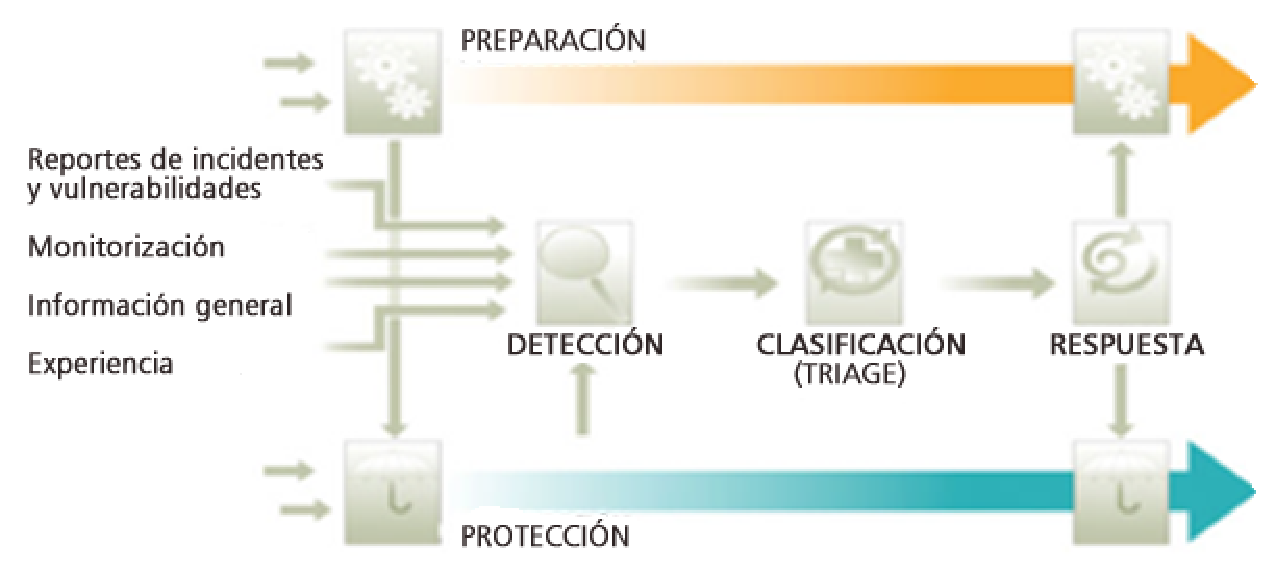
\includegraphics[scale=0.4]{./img/1-gis}
\caption{Modelo de precesos para Gestión de Incidentes de Seguridad (GISeg)}
\end{figure}


Para dar una idea de la complejidad del problema de procesamiento de alertas por parte de los analistas para alcanzar el CS, actividades vinculadas principalmente a los procesos 3 y 4 del modelo, basta mencionar un simple ejemplo en el que la tasa de producción de alertas de dispositivos con un grado medio de sintonización puede estar entre 750 y 1000 alertas diarias para un esquema básico de tres sensores (2xHIDS, 1xNIDS) monitorizando 7 aplicaciones Web de Internet sobre un esquema de arquitectura de red con una única DMZ.

Además de la problemática vinculada al tratamiento de grandes volúmenes de datos, el proyecto plantea una serie de desafíos a superar vinculados directamente con el área de AV:

\begin{enumerate}
\item {\bfseries Sobrecarga de información:} El problema plantea el procesamiento de una gran cantidad de datos con una tendencia acentuada en el incremento del volumen a mediano plazo. Además, los tipos de datos manejados suelen ser dispares y cambiantes. 
\item {\bfseries Tamaño de pantallas limitado:} Existe un problema respecto a la presentación de los datos ya que se cuenta con espacio limitado en los monitores. Esto significa que muchas veces no resulta posible presentar toda la información en una pantalla al mismo tiempo. Para esto debe pensarse en técnicas de fusión y modelado de datos. 
\item {\bfseries Análisis de datos heterogéneos:} Distintos dominios de conocimiento generan distintos tipos de información, en muchos casos en tiempo real, como ser registros de actividad (logs) y alertas vinculados con aplicaciones, sensores, bases de datos, etc. 
\item {\bfseries Interpretación de información:} Es necesario generar una salida uniforme y entendible a partir de una aplicación analítica. La forma de interpretar los datos depende principalmente de la calidad de los mismos.
\item {\bfseries Semántica:} Otro desafío es el de proveer una significado lógico uniforme para todos los datos que se están analizando y presentando a los analistas.
\end{enumerate}



\section{Solución y Prototipo}

Dar solución a las problemáticas planteadas enla sección anterior requiere previamente de un estudio del rol de los diferentes actores intervinientes en el problema de seguridad en infraestructuras de TIC por lo que deben ser analizados tanto los componentes objetivo de ataques y sus aplicaciones y servicios vinculados, como los atacantes, sus organizaciones, motivaciones, ubicación geográfica, herramientas utilizadas, y si resulta posible sus motivaciones y relaciones.

El problema será abordado por medio de la explotación de técnicas de análisis visual y fusión de datos que soporten el procesamiento de grandes volúmenes de alertas de seguridad generadas por dispositivos vinculados a estructuras de protección. Debido a la naturaleza compleja del problema y a las fuertes limitaciones de las técnicas y herramientas tradicionales de análisis, se ha decidido avanzar en el diseño y desarrollo de una solución que genere una reducción sensible en la tensión cognitiva del analista por medio de la utilización de análisis visual para favorecer su capacidad de  percepción. En el procesamiento perceptivo se combinan el color, la figura de fondo, la constancia de la forma, la representación y el análisis perceptivo visual del hemisferio derecho del cerebro. Resulta fundamental para el éxito de la propuesta la comprensión de la manera en que la percepción y la cognición afectan a la visualización de la información con el fin de optimizar la manera de presentar la información por medio de interfaces adecuadas. A tal fin se considerarán resultados relevantes de las teorías existentes de la psicofísica y su relevancia científica en la visualización de información.

\subsection{Requerimientos del prototipo}

Para el desarrollo del prototipo se pensó en una serie de requerimientos, los cuales pueden ser agrupados en dos tipos: funcionales y visuales.

Con respecto a los requerimientos funcionales el sistema debe:

\begin{enumerate}
\item Facilitar el CS, 
\item Permitir la agregación y la normalización de datos, 
\item Ser orientado a Web (accesibilidad, servicios, etc.), 
\item Contar con los mecanismos de seguridad correspondientes (AAA),
\item Permitir de correlación de alertas,
\item Permitir la generación de escenarios futuros a partir de información actual,
\item Explotar la representación de información de eventos en base a modelos que faciliten el análisis.   \newline

Respecto a los requerimientos visuales: 

\item El sistema debe contar con una interfaz gráfica única, 
\item La interfaz debe permitir al operador generar un modelo mental del problema, 
\item La interfaz debe ser interactiva facilitando el proceso de análisis, 
\item La representación visual debe permitir el CS.
\end{enumerate}


\subsection{Aproximación a la Solución}

La definición de CS mas relevante a los objetivos del presente trabajo puede sintetizarse de la siguiente manera: CS consiste en la percepción de los elementos en un dominio determinado, dentro de un volumen determinado de tiempo y espacio, la comprensión de su significado, y la proyección de su situación en el futuro cercano \cite{b2}.

Según Endsley, percepción, comprensión y proyección conforman los tres pilares fundamentales de CS. A continuación se presentan los componentes del modelo de CS, y mas abajo en la Figura 2 un esquema de los componentes vinculados a CS del mismo:

\begin{enumerate}
\item Percepción (Nivel 1 CS): construcción de los elementos más básicos de CS, principalmente asociado al estado, características o atributos y dinámica de los diferentes actores en el modelo (personas, objetos, eventos, ambiente, etc.). Se basa en procesos de monitorización, detección y reconocimiento. 
\item Comprensión (Nivel 2 CS): implica una síntesis de los elementos generados por el Nivel 1 CS. Se utilizan técnicas de reconocimiento de patrones, interpretación y evaluación. En esencia, el Nivel 2 debe facilitar la identificación del impacto de las variables relevantes de modelo en los objetivos y metas de cada uno de los componentes. 
\item Proyección (Nivel 3 CS): capacidad de anticipar la posible evolución del modelo, es decir predecir el comportamiento de los diferentes elementos del mismo. Se explota la información producida en los Niveles 1 y 2 con el objetivo de predecir comportamientos, acciones.
\end{enumerate}


\begin{figure}
\centering
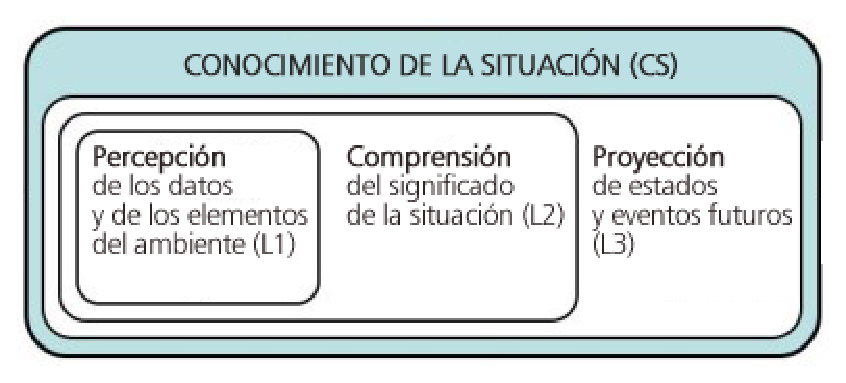
\includegraphics[scale=0.5]{./img/1-cs}
\caption{Componentes CS del Modelo de Endslay}
\end{figure}

Si bien existen mecanismos alternativos para la reducción de los volúmenes de información como por ejemplo los lenguajes de correlación como LUA \cite{b3}, y otros \cite{b4} \cite{b5} \cite{b6}, y la asistencia mediante sistemas inteligentes \cite{b7} \cite{b8} \cite{b9} \cite{b10}, en este trabajo se probará la potencialidad del AV. 



\subsection{Normalización de Datos}

Como parte del preprocesamiento se prevé la agregación y normalización de la totalidad de alertas almacenadas en las bases de datos. El formato seleccionado para normalización es el Formato de Mensajes de Intercambio de Alertas de Intrusión (IDMEF) \cite{b11} desarrollado por el Grupo de Trabajo sobre Detección de Intrusos de la IETF. IDMEF ha sido concebido para permitir que las diferentes tecnologías de detección y los productos de distintos fabricantes puedan interoperar mediante el intercambio de información de alertas de seguridad.


\subsection{Comunicación Cliente/Servidor}

La solución propuesta debe prever mecanismos eficientes para soportar la comunicación entre el cliente y el núcleo de la aplicación en el que se centra el procesamiento de datos, por lo que se ha optado por una arquitectura de software de tipo Modelo Vista Controlador (MVC), en la que el 100% de la vista funciona sobre un navegador Web. La principal problemática para el presente caso de aplicación del modelo MVC se plantea en término de tasa de transferencia de datos debido a la gran cantidad de información que debe ser transferida con el objetivo de mantener una representación visual lo mas real posible con características lo mas cercanas posibles a sistemas de tiempo real. La solución a este problema ha sido abordada mediante la utilización de un formato ligero de intercambio de datos basado en el JavaScript Object Notation (JSON) \cite{b12}.

\subsection{Vector de Representación}

Resulta indispensable al momento de presentar gráficamente un evento de seguridad la correcta identificación de los componentes básicos involucrados. Se realiza una primera aproximación a dichos componentes en base al trabajo realizado en Visalert \cite{b13} el cuál se basa en la premisa de que los sistemas de análisis deben aprovechar tres atributos fundamentales para lograr una base sólida de correlación. A esta premisa se la denomina {\bfseries  qdc} debido a las siglas de que, donde y cuando: \newline
{\bfseries ¿Que?:} qué tipo de ataque \newline
{\bfseries ¿Donde?:} cuál es el objetivo  \newline
{\bfseries ¿Cuando?:} cuándo se realizó el ataque \newline

Si bien la premisa establecida originalmente resulta válida para aspectos puramente analíticos desde la perspectiva de los objetivos de ataque donde la pregunta relevante es: ¿que es lo que está ocurriendo en un determinado momento con los diferentes activos de TIC?, se considera que el modelo carece de componentes que podrían considerarse elementales para sistemas de protección. En el presente trabajo se propone el agregado de una serie de componentes a la premisa qdc que se cree aportan gran valor al modelo final, sobre todo en ambientes de defensa e inteligencia en los que resulta imprescindible conocer e identificar el origen de las acciones ofensivas y su clasificación de tal manera que puedan emprenderse acciones disuasivas, legales e incluso contraofensivas. \newline

El nuevo modelo debería prever la posibilidad de establecer: \newline
- Identificación del atacante, \newline
- Identificación de grupos o alianzas hostiles, \newline
- Identificación de la fuente de los ataques, \newline
- Herramientas utilizadas, \newline
- Nacionalidades, y \newline
- Alianzas o relaciones, etc. \newline
	
Al conjunto de elementos a representar vinculados a un determinado evento de seguridad se lo denomina en adelante como Vector de Representación (VR). Cada VR está asociado a una alerta en el sistema de fusión. \newline

Se prevé además la posibilidad de generar Meta Vectores de Representación en base a la fusión o clustering de VR individuales.
	

\subsection{Componentes del Vector}
    

A continuación se definen los componentes de los VR para el sistema propuesto y la asignación de los componentes de identificación según el esquema adoptado de normalización de datos en base a IDMEF. \newline
Para la premisa inicial (qdc) los componnetes son: 
\begin{enumerate}
\item Que (classification, assessment, additional\_data) 
\item Donde (target information: ip address, name, location)
\item Cuando (create\_time, analyzer\_time, detect\_time)
\end{enumerate}

Como aporte del presente trabajo de investigación, a la premisa original se suman al modelo tres nuevos componentes:
\begin{enumerate}
\setcounter{enumi}{3}
\item Quién (source information: ip address, country)
\item Dispositivo (analyzer information: type, name)
\item Carga útil o payload (additional\_data, message, severity, impact)
\end{enumerate}




La nueva premisa para el sistema queda definida como {\bfseries qdc2}: {\itshape que, donde, cuando, quién, dispositivo, y carga}. Este nuevo aporte (quién, dispositivo, carga) permite detectar el origen del ataque (dirección ip, país) y detalles de la misma, concentrando información respecto a la criticidad de la alerta, el impacto en la infraestructura, y características particulares del evento.

Debido al carácter relacional de los VR se ha tomado la decisión de utilizar Grafos para el desarrollo de los componentes fundamentales de la herramienta de AV. Los grafos junto a la fusión de datos facilitan la representación de gran cantidad de información por medio de la vinculación directa e indirectamente todos los componentes del VR por medio de nodos y relaciones entre ellos.


\subsection{Implementación del Prototipo de Producción}

La implementación del prototipo fue llevada adelante como una capa extra de servicio en la arquitectura de protección de redes de Bacchuss \cite{b14}. En la Figura 3 se detallan los componentes definidos en esta instancia de investigación para cada uno de los componentes del VR:

\begin{figure}
\centering
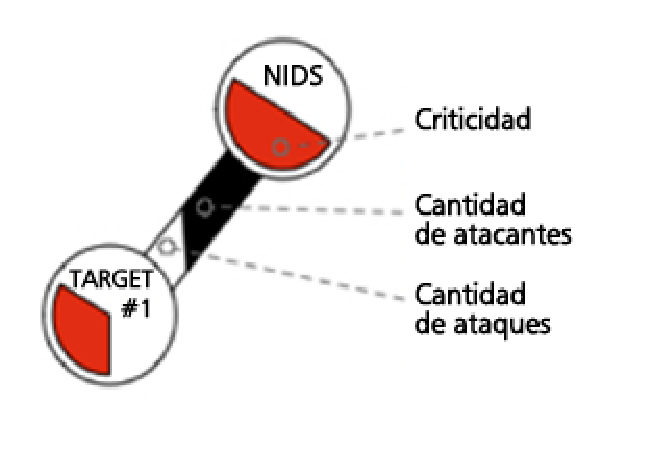
\includegraphics[scale=0.5]{./img/1-mp2}
\caption{Componentes del Ventor de Representación}
\end{figure}

El modelo de representación seleccionado permite representar diversas variables relevantes del problema en la estructura de grafos subyacente. En base a este concepto se procede a continuación a describir sintéticamente los diferentes componentes visuales asociados a los VR, los cuales responden a requerimientos de AV. 


Primero, la criticidad de un nodo (nivel de riesgo) se establece en función a la criticidad de su categoría superior. La función matemática necesaria para dicha representación es, en este caso, una función directa. Ej.: si del total de alertas recibidas el 50\% son consideradas críticas, entonces se pinta el 50\% del nodo en color rojo. Segundo, la cantidad de ataques representa el total de alertas recibidas en un momento dado, y se muestra como la relación entre los nodos, dibujando este vínculo con mayor o menor espesor en función a la cantidad de alertas. La función matemática utilizada es, en este caso, de relación directa: cuantas más alertas se reciben, más ancha se dibuja la relación. Tercero, la cantidad de atacantes involucrados en un momento dado, viene establecido como el nivel de relleno del eje de relación entre dos nodos mencionado en el párrafo anterior. Se calcula el relleno de la relación de la misma manera en que fue calculada la cantidad de alertas. Esta forma de representación visual de eventos en base a la modularización de las funciones de peso permite ensayar el sistema con diferentes funciones matemáticas y ver los resultados.


El prototipo presenta la información en un formato de círculos concéntricos denominados niveles, siempre en base a estructuras de grafos, donde cada nivel es asociado a un tipo relevante de datos del VR propuesto. En la Figura 4 se representa hasta el nivel \#4 del sistema, donde: \newline
- nivel \#0: representa al objeto de protección (blanco), \newline
- nivel \#1: representa el tipo de tecnología de detección (HIDS, NIDS), \newline
- nivel \#2: producto utilizado para la detección (Snort, OSSEC), \newline
- nivel \#3: clasificación del tipo de evento (ataque-Web, dos, gusano, etc.), y \newline
- nivel \#4: datos asociados al tipo de evento, detalles técnicos. \newline

\begin{figure}
\centering
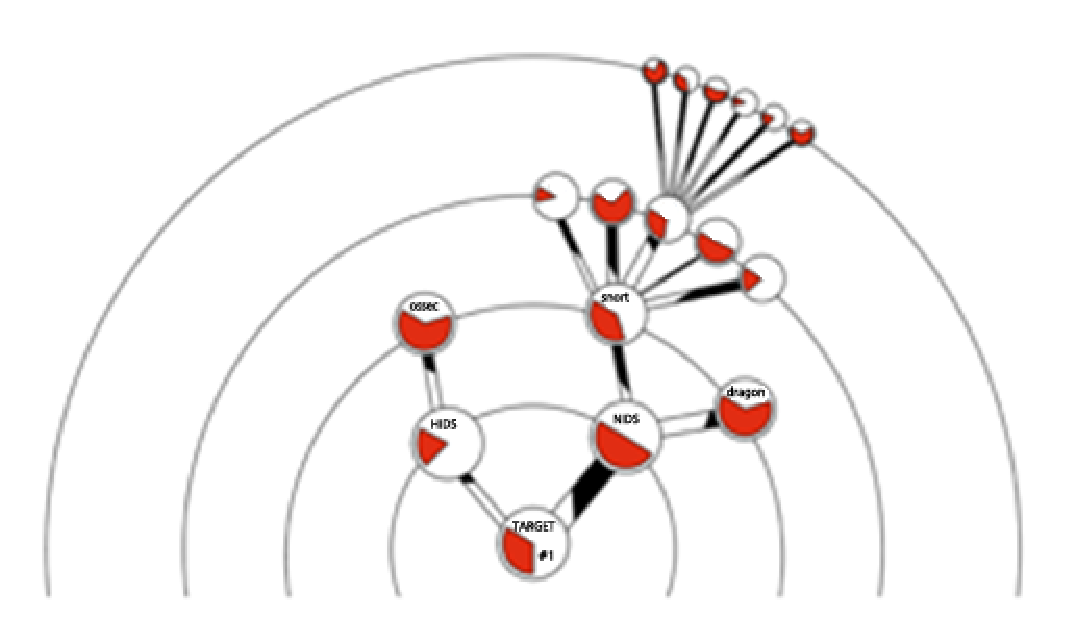
\includegraphics[scale=0.55]{./img/1-mp3}
\caption{Mapa de Niveles de Representación}
\end{figure}



Es importante considerar que una de las técnicas utilizadas para la reducción de los volúmenes de información consiste en el agrupamiento de eventos con características similares. Por ejemplo, el prototipo prevé la representación en pantalla de alertas agrupadas en categorías, indicando la criticidad de estas últimas, el sensor relacionado, datos de la tecnología soporte y finalmente la criticidad del objetivo. Para poder analizar diferentes situaciones se han contemplado además una serie de escalas temporales que permiten aumentar o reducir la cantidad de eventos procesados por la herramienta. En esta instancia se han definido las siguientes escalas: {\itshape alertas generadas en último día; en la última semana; en el último mes; en los últimos 3 meses; y en los últimos 6 meses}.

En la Figura 5 puede verse una captura de un escenario real de aplicación del sistema para una cantidad de 150000 alertas generadas por medio de la simulación de ataques con soporte en usuarios sintéticos.

\begin{figure}
\centering
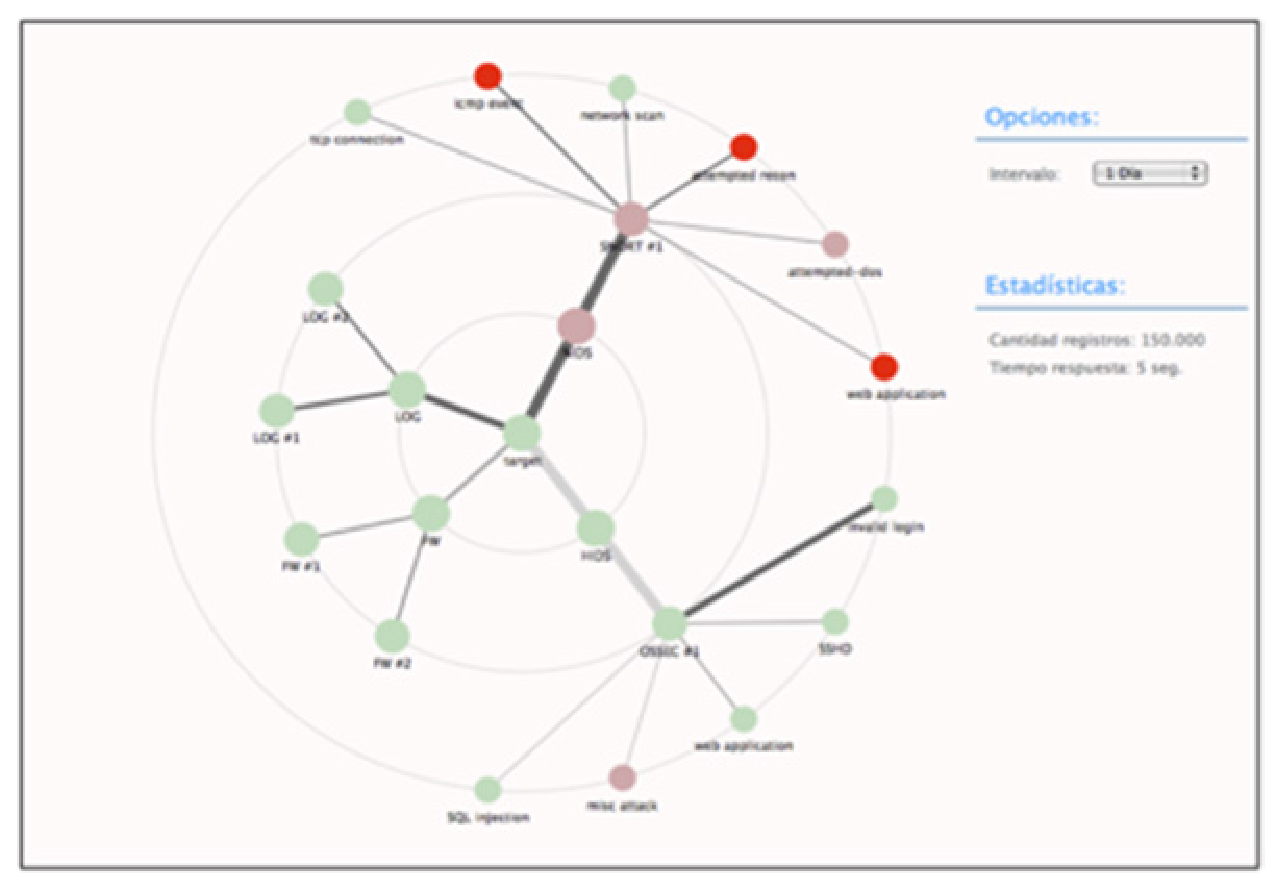
\includegraphics[scale=0.46]{./img/1-mp4}
\caption{Captura del Prototipo en Funcionamiento}
\end{figure}


Del lado derecho de la imagen se visualizan los filtros según intervalo de tiempo. En el centro se puede observar el resultado del procesamiento de las alertas. Los nodos rojos representan nodos críticos, nodos que se encuentran expuestos a niveles elevados de riesgo. Los nodos color salmón representan una criticidad media; y finalmente los nodos de color verde claro representan nodos no críticos. Las relaciones entre los nodos varían en espesor e intensidad de color según lo explicado en secciones anteriores. Las relaciones finas y claras representan pocas alertas y no críticas. Las relaciones van aumentando en su espesor según vayan creciendo la cantidad de alertas generadas. El color se torna más oscuro en función a la relación alerta-atacante. \newline 

En cuanto a los resultados experimentales, la finalización reciente del prototipo funcional no ha permitido la simulación de casos reales. Las pruebas realizadas al momento fueron orientadas principalmente a la verificación del cumplimiento de los requerimientos estructurales y funcionales de la herramienta, aunque algunos de los resultados obtenidos evidencian ya la potencialidad de la herramienta como instrumento de soporte para los analistas de seguridad. 


\section{Conclusiones y Trabajo Futuro}

El uso técnicas de análisis visual y fusión de datos resultan de gran utilidad al momento de soportar herramientas de CS para la optimización de los procesos de toma de decisión. Mediante el estudio del proceso de cognición y percepción del ser humano, y haciendo uso de herramientas y técnicas visuales en conjunto con la implementación de grafos, se ha demostrado que se puede disminuir la tensión cognitiva del analista de seguridad con el fin de interpretar la realidad y formar un modelo mental de la situación lo que deriva en una mejor toma de decisiones. \newline

La herramienta desarrollada resulta de especial interés en escenarios de defensa para grandes infraestructuras de TIC, especialmente para incidentes conformados por múltiples ataques individuales. Por ejemplo, resulta de gran interés experimental el tratamiento de amenazas planteadas por gusanos y nuevas herramientas cuyos algoritmos de propagación son altamente eficientes en términos de propagación y tiempos de infección, y cuyas cargas efectivas de datos son altamente manejables lo que permite convertirlos en herramientas ofensivas. \newline

Con respecto al trabajo futuro, quedan pendientes la aplicación del prototipo a diversos escenarios reales con el objetivo de ganar experiencia y descubrir su valor y potencialidad, la exploración de la representación de datos almacenados sobre modelos de grafos, la utilización de inteligencia artificial para la proyección de escenarios a futuro, y la posibilidad de correlacionar la información del modelo referida a niveles de criticidad de los nodos con datos de validación de vulnerabilidades asociadas a los diferentes activos de TIC sujetos de protección.







\begin{thebibliography}{4}

\bibitem{b1} Ramon Mosso, J.M.: Modelo de Gestión de Incidentes de Seguridad (2008). Bacchuss.

\bibitem{b2} Endsley, M.R.: Toward a theory of situation awareness in dynamic systems. Human Factors 37(1), 32–64. (1995)

\bibitem{b3} LUA programming Languaje. \url{http://www.lua.org/about.html}

\bibitem{b4} Abadyz C., Taylory J., Senguly C., Yurcikz W., Zhouy Y., Rowex K.: Log Correlation for Intrusion Detection: A Proof of Concept.

\bibitem{b5} Kruegel C., Valeur F., Vigna G.: Intrusion Detection and Correlation - Challenges and Solutions.
Series: Advances in Information Security, Vol. 14 (2005)

\bibitem{b6} Cuppens F., Miège A.: Alert Correlation in a Cooperative Intrusion Detection Framework
ONERA Centre de Toulouse, 2, av. Edouard Belin, 31005, Toulouse CEDEX, France

\bibitem{b7} Frank J.: Artificial Intelligence and Intrusion Detection: Current and Future Directions
Division of Computer Science, University of California at Davis, 1994.

\bibitem{b8} Manninen M.: Using Artificial Intelligence in Intrusion Detection Systems
Helsinki University of Technology

\bibitem{b9} Sadkhan S.B.: On Artificial Intelligence Approaches for Network Intrusion Detection Systems
MASAUM Journal of Computing, Volume 1 Issue 2 (2009).

\bibitem{b10} Morel B.: Anomaly Based Intrusion Detection and Artificial Intelligence 
Publisher: InTech (2011)

\bibitem{b11} Debar H., Curry D., Feinstein B.: “The Intrusion Detection Message Exchange Format” (2006)

\bibitem{b12} JavaScript Object Notation (JSON). \url{http://json.org/json-es.html}

\bibitem{b13} Livnat Y., Agutter J., Moon S., Erbacher R., Foresti S.: A Visualization Paradigm for Network Intrusion Detection (Visalert)

\bibitem{b14} Sistema de Gestión de Incidentes de Seguridad (2008). Bacchuss. 

\end{thebibliography}


\end{document}
